%%% template.tex
%%%
%%% This LaTeX source document can be used as the basis for your technical
%%% paper or abstract. Intentionally stripped of annotation, the parameters
%%% and commands should be adjusted for your particular paper - title, 
%%% author, article DOI, etc.
%%% The accompanying ``template.annotated.tex'' provides copious annotation
%%% for the commands and parameters found in the source document. (The code
%%% is identical in ``template.tex'' and ``template.annotated.tex.'')

\documentclass[annual]{acmsiggraph}

\TOGonlineid{45678}
\TOGvolume{0}
\TOGnumber{0}
\TOGarticleDOI{1111111.2222222}
\TOGprojectURL{}
\TOGvideoURL{}
\TOGdataURL{}
\TOGcodeURL{}

\usepackage{caption}
\usepackage{subcaption}
\usepackage[english]{babel}
\title{Goes Here}

\author{}
\pdfauthor{}

\keywords{}

\begin{document}

 \teaser{
   \begin{subfigure}[b]{0.3\textwidth}
	\centering
    	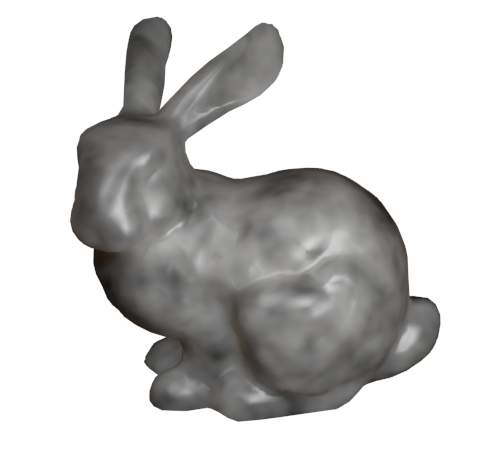
\includegraphics[width=0.6\textwidth]{figure/bunny_orig.png}
      	\caption{}
        \label{teaser:original}
        \end{subfigure}
        ~ 
        \begin{subfigure}[b]{0.18\textwidth}
                \centering
    	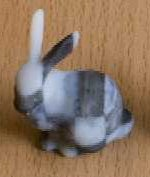
\includegraphics[width=\textwidth]{figure/bunny_print1.jpg}
                \caption{}
                \label{teaser:ours}
        \end{subfigure}
        ~
        \begin{subfigure}[b]{0.2\textwidth}
                \centering
    	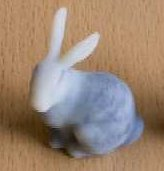
\includegraphics[width=\textwidth]{figure/bunny_print2.jpg}
                \caption{}
                \label{teaser:makerbot}
        \end{subfigure}
        ~
        \begin{subfigure}[b]{0.18\textwidth}
                \centering
    	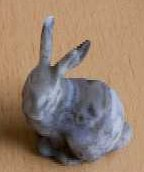
\includegraphics[width=\textwidth]{figure/bunny_print3.jpg}
                \caption{}
                \label{teaser:objet}
        \end{subfigure}
        \caption{A textured mesh printed with different types of 3D printers.
        	(a)original model.(b)printed with our printer.(c)makerbot.
        	(d)objet}\label{teaser}
 }

\maketitle

\begin{abstract}


\end{abstract}

\keywordlist

\TOGlinkslist

\copyrightspace

\section{Introduction}
3D printing has the potential to dramatically reduce the required time and cost of
fabricating custom materials and objects. In particular, it allows the fabrication of materials with complex internal
structures that are difficult or impossible to manufacture with other technologies. Additive manufacturing could be
much more widely adopted and easier to use, given a high-fidelity translation from specifications of objects defined
in terms of their mechanical, optical, and appearance properties to output-device-specific computer
programs that produce the best possible approximation of these digital objects. However, this is still one of
the most important unsolved problems in digital direct manufacturing. Due to its combinatorial nature, this
problem becomes more and more challenging as the range of different printable materials increases. This paper
aims to provide an abstraction mechanism and a software framework for translating specifications to fabrication
instructions. It is possible to design a computationally efficient and general process for translating virtual objects
with desired mechanical, electrical, optical, and appearance properties into composite printable materials.
We will achieve this goal through a reduction-optimization-simulation approach.
\section{Previous Work}
\subsection{Simulation of the Appearance of Ink Combinations}
\cite{Matusik:2009} built a system
for the measurement of Bidirectional Reflectance Distribution Functions (BRDFs) and were able
to acquire BRDFs for both single-layer and multi-layer ink printouts (e.g., an ink covered by a
varnish layer). They then acquired a database of many different combinations of ink layers (up to
seven layer combinations were considered). However, they did not develop a method to simulate
the appearance of arbitrary ink layers. They were able to interpolate the appearance by spatially
multiplexing small tiles of different base combinations. By linearity of light transport, the simulation
of the combined appearance was reduced to linear combinations of the base BRDFs. 
simulation method for the appearance of translucent materials \cite{Hasan:2010}. 
They
built a measurement system for estimating multiple-scattering in homogeneous material slabs. They
measured both transmission and refection for a set of base materials used by the OBJET Connex
multi-material printer. 
Using these measurements, our simulations framework was able to predict
diffuse reflections and transmissions in multi-layered translucent objects composed of base material
layers.
In the proposed research, we will extend these methods to cover the complete appearance of
volumetric materials that accounts for both directly reflected light and light scattering within the
material volume. 
We will use efficient simulation methods that allows us to simulate the appearance
of complex structures composed from these base materials. We developed an initial framework for
simulating behavior of multi-layered materials, where each layer is a homogeneous base material.
Then we extend this simulation to materials in which each voxel is made of a different measured
material. Since this general simulation is expensive and requires path-tracing algorithms, we used
algorithms that are based on fast numerical integration of our low-dimensional representations
and the use of pre-computation, similar to pre-computed light transport approaches \cite{Sloan:2002}.
\subsection{Simulation of Deformation Behavior}
In previous work, the problem
of modeling and simulating soft materials and their deformation behavior \cite{Bickel:2010,Bickel:2009}.
In order to accurately model deformation behaviors they built a system that allowed measuring how
a given material deforms subject to a variety of external forces. 
The system used an automated
robot arm to apply desired forces and a vision subsystem to measure corresponding surface deformations.
We modeled deformation behavior of a material using a stress-strain relationship. Since
the deformation behavior of many of our materials was non-linear, we developed a model that could
accurately represent this behavior and that was also easy to fit to the surface measurements. In
our model, the stress-strain relationship was represented as a collection of linear stress-strain relationships.
We used a properly chosen function to interpolate between these linear relationships
and obtain a non-linear model. Using this system and model we could accurately measure material
deformation of a collection of materials produced by a multi-material printer and fit these observation
to the stress-strain model. Then, using this material model within a Finite Element Method
we could accurately simulate behavior of any shape made from a composite of measured materials.
In the proposed research, we would like to address the shortcomings of our current measurement
and models. First, our current approach handles only elastic material deformation. We would like to
extend our current data-driven model to viscoelastic materials. In fact, most real materials exhibit
this property, which is characterized by hysteresis (or material memory). For these materials, it is
not possible to predict the behavior of a material only based on the currently applied stress. One also
has to know the history (or the sequence) of applied stress values to accurately simulate material
behavior. In order to determine the material model one has to measure the so called hysteresis
loops in the stress-strain space (as opposed to a single stress-strain curve for elastic materials). The
hysteresis loop is the result of the damping effect which causes the material to behave differently
depending whether stress is applied or removed as some of the energy is dissipated within the
material into heat. Additional advantage of using this material model is that it will allow us to
handle dynamic material deformations.

In order to measure viscoelastic material properties, we will need to modify our current measurement
system and procedures. We will use repeatable, time-coded measurements to estimate
Figure 5: From left to right: Force-and-deformation capture of a non-linear heterogeneous pillow;
synthesized deformation with fitted material parameters; and interactive deformation synthesized
with our soft tissue modeling technique using scattered data interpolation \cite{Bickel:2010}.

We will also use faster resonating actuators and high-speed
camera systems to track material deformations at high frame rates. Furthermore, we plan to track
the whole material volume rather than the outer material surface. This is possible since we can
print materials in clear color as well. Thus small color-coded markers can be easily embedded into
the material structure. These markers can be tracked in 3D using a multi-camera system.
\section{System Description}
The software framework (shown in Figure~\ref{fig:framework}) is composed of 
a set of software
modules that can be easily modified or exchanged. The first component
of this framework is an output-device-independent description API
that allows the user to specify any physical object in terms of its physical
properties such as geometry, mechanical behaviors, and appearance. 
The framework will also provide physically-based
simulation tools that accurately predict the behavior of our output device.
The goal of the optimization module is to search through
the space of possible device outputs and deliver one that best matches the
desired model. In order to evaluate the quality of the match between the
simulation output and the desired model we need to develop appropriate
comparison metrics. Finally, a central component of our framework is
a reduction model which makes the optimization problem tractable by
reducing the search space as much as possible.
The reduction model can specified by experts or deduced from a
set of examples. Next, we will describe each element of the framework in
more detail.
\begin{figure}
\caption{API overview}
\label{fig:framework}
\end{figure}
\subsection{Input API}
Our input API allows a designer to either
define material properties for sections of an object
or specify behavior of an object. 
The designer
can use functions to describe properties such as reflectance (e.g., BRDFs, BSSRDFs), 
stiffness, or other spatially varying properties. 
Although it is possible to define the object directly by only specifying material
properties, intuitive user
interfaces will aid in specifying the objects and their properties
in terms of intuitive metaphors.
For example, the elastic properties of an object can be specified by a set of
example displacements from the rest pose and the corresponding applied forces.
\subsection{Search Space Decomposition and Reduction}
Our framework includes an optimization component that
searches through the space of possible device inputs
to find the one that best reproduces
the desired object. Unfortunately, this search space
is usually high-dimensional. For example, when the printing
volume has N voxels and each of these voxels can be
assigned to one of M base materials, the search space
has $N^M$ dimensions. To overcome this problem, we decompose the search
space into similar subproblems and also reduce
the search space to a lower-dimensional space using
a reduction model. The goal of the reduction step is to
shrink the search space as much as possible but at the
same time not to prune out good solutions. The low-dimensional space produced by the
reducer can be defined in two different ways. First, a reduction model can be explicitly specified by an expert, for
example, by defining structures of base materials and rules how different base materials can be combined together.
The second way to specify a reduction model is implicit. In this case, the user provides a set of examples of
valid material structures. Then, a machine learning algorithm infers both basic material structures and the rules
for combining them. The optimization framework can be further improved by employing techniques that cluster
partial solutions that yield similar output properties, avoiding combinatorial explosion of the search space.
Furthermore, we can employ bounds on the solution based on physical constraints of the base materials.
\subsection{Optimization}
Our optimization component is an interface to 
existing standard optimization techniques
such as simulated annealing, genetic algorithms and
Markov Chain Monte Carlo methods, as well as custom optimization algorithms implemented
by more advanced users.
\subsection{Simulation}
Another key step in the process of converting abstractions to physical output is being able to
simulate what an output device is going to generate given a well-defined input. 
A simulation allows the user to preview how the output will look and behave. 
This simulation is a generalization of the print-preview function
available in word processing applications.
As physical output generation might be costly or time-consuming, 
it is extremely beneficial for users to be able to preview the output and make immediate changes to the design.
That means that the simulation must accurately predict the output. 
It's necessary to develop very efficient and accurate rendering
and finite element simulation packages. Since we run the simulation multiple times within the optimization method
we can cache and reuse partial simulation results, speeding up the evaluation process at least 10-100 times.
Furthermore, we will ensure that the simulation is accurate by measuring properties of the printing materials and using
these measurements to estimate the parameters of data-driven material models (e.g., for elasticity, reflectance).
\section{Programming with Our API}
Code examples:
To generate textured model:
\begin{verbatim}
Manager manager;
manager.loadMaterialLib("material_file");
manager.setGenerator(
  new HeightFieldGenerator());
manager.setSimulator(colorSimulator());
manager.setMetric(someColorMetric());
manager.setOptimizer(
  simulatedAnealing);
  //or e.g. gradientDescent
Objective obj;
Scene scene;
TexturedShape shape("filename");
TexturedShape goal("filename1");
scene.addShape(shape);
obj.setScene(scene);
obj.setGoal(goal);
manager.addObjective(obj);
\end{verbatim}

To generate BRDF
\begin{verbatim}
manager.setGenerator(stackingGenerator);
manager.setSimulator(brdfSimulator);
manager.setMetric(someImageMetric);
Shape shape("filename"), 
Image goal("filename1");
\end{verbatim}

Deformation
\begin{verbatim}
force = new Force(pos, dir, shapeID);
constraint = new Constraint(
    FIX_VERTEX, vertexList, shapeID));

scene.addForce(force);
scene.addConstraint(constraint);
Shape goal;
manager.setSimulator(femSimulator);
\end{verbatim}

\section{Experiments}
\subsection{Previous Work}
Subsurface scattering. Mechanical properties
A figure showing a material with a particular
look and deformation properties is shown in Figure~\ref{fig:deform}

\begin{figure}
\begin{subfigure}[b]{0.3\textwidth}
	\centering
 	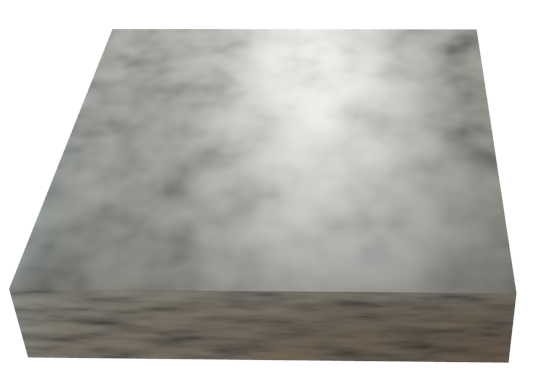
\includegraphics[width=\textwidth]{figure/slab_origin.png}
   	\caption{}
    \label{fig:deformPhoto}
    \end{subfigure}
    ~ 
    \begin{subfigure}[b]{0.3\textwidth}
    \centering
  	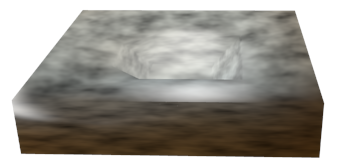
\includegraphics[width=\textwidth]{figure/slab_deform.png}
    \caption{}
    \label{fig:deformPrint}
\end{subfigure}
\caption{Simutaneously matching appearance and deformation. 
(a)Original slab of a particular looking. (b)printed slab 
with the same looking and desired deformation.}
\label{fig:deform}
\end{figure}

Two error plots showing subsurface scattering and deformation errors decrease
after each iteration in Figure~\ref{fig:err}.

\begin{figure}
\begin{subfigure}[b]{0.3\textwidth}
	\centering
 	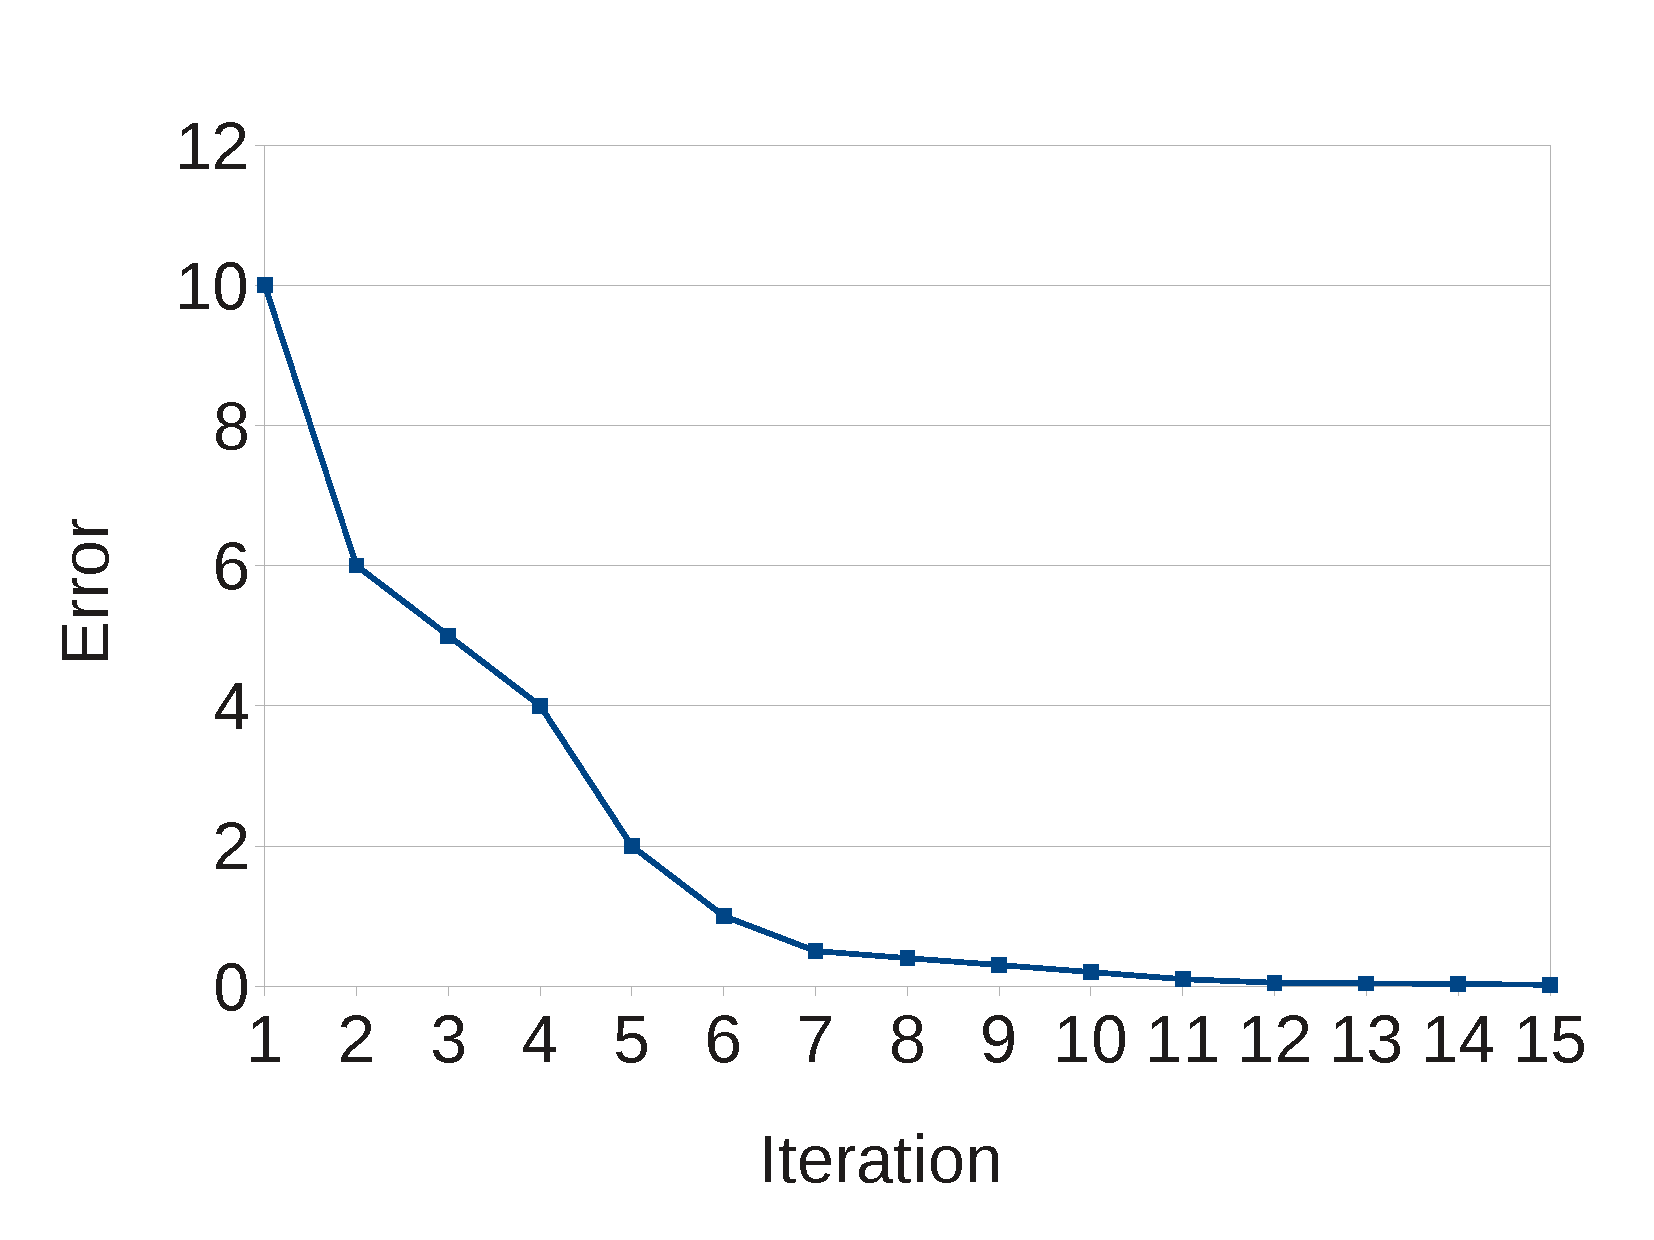
\includegraphics[width=\textwidth]{figure/error.pdf}
   	\caption{}
    \label{fig:ssErr}
    \end{subfigure}
    ~ 
    \begin{subfigure}[b]{0.3\textwidth}
    \centering
  	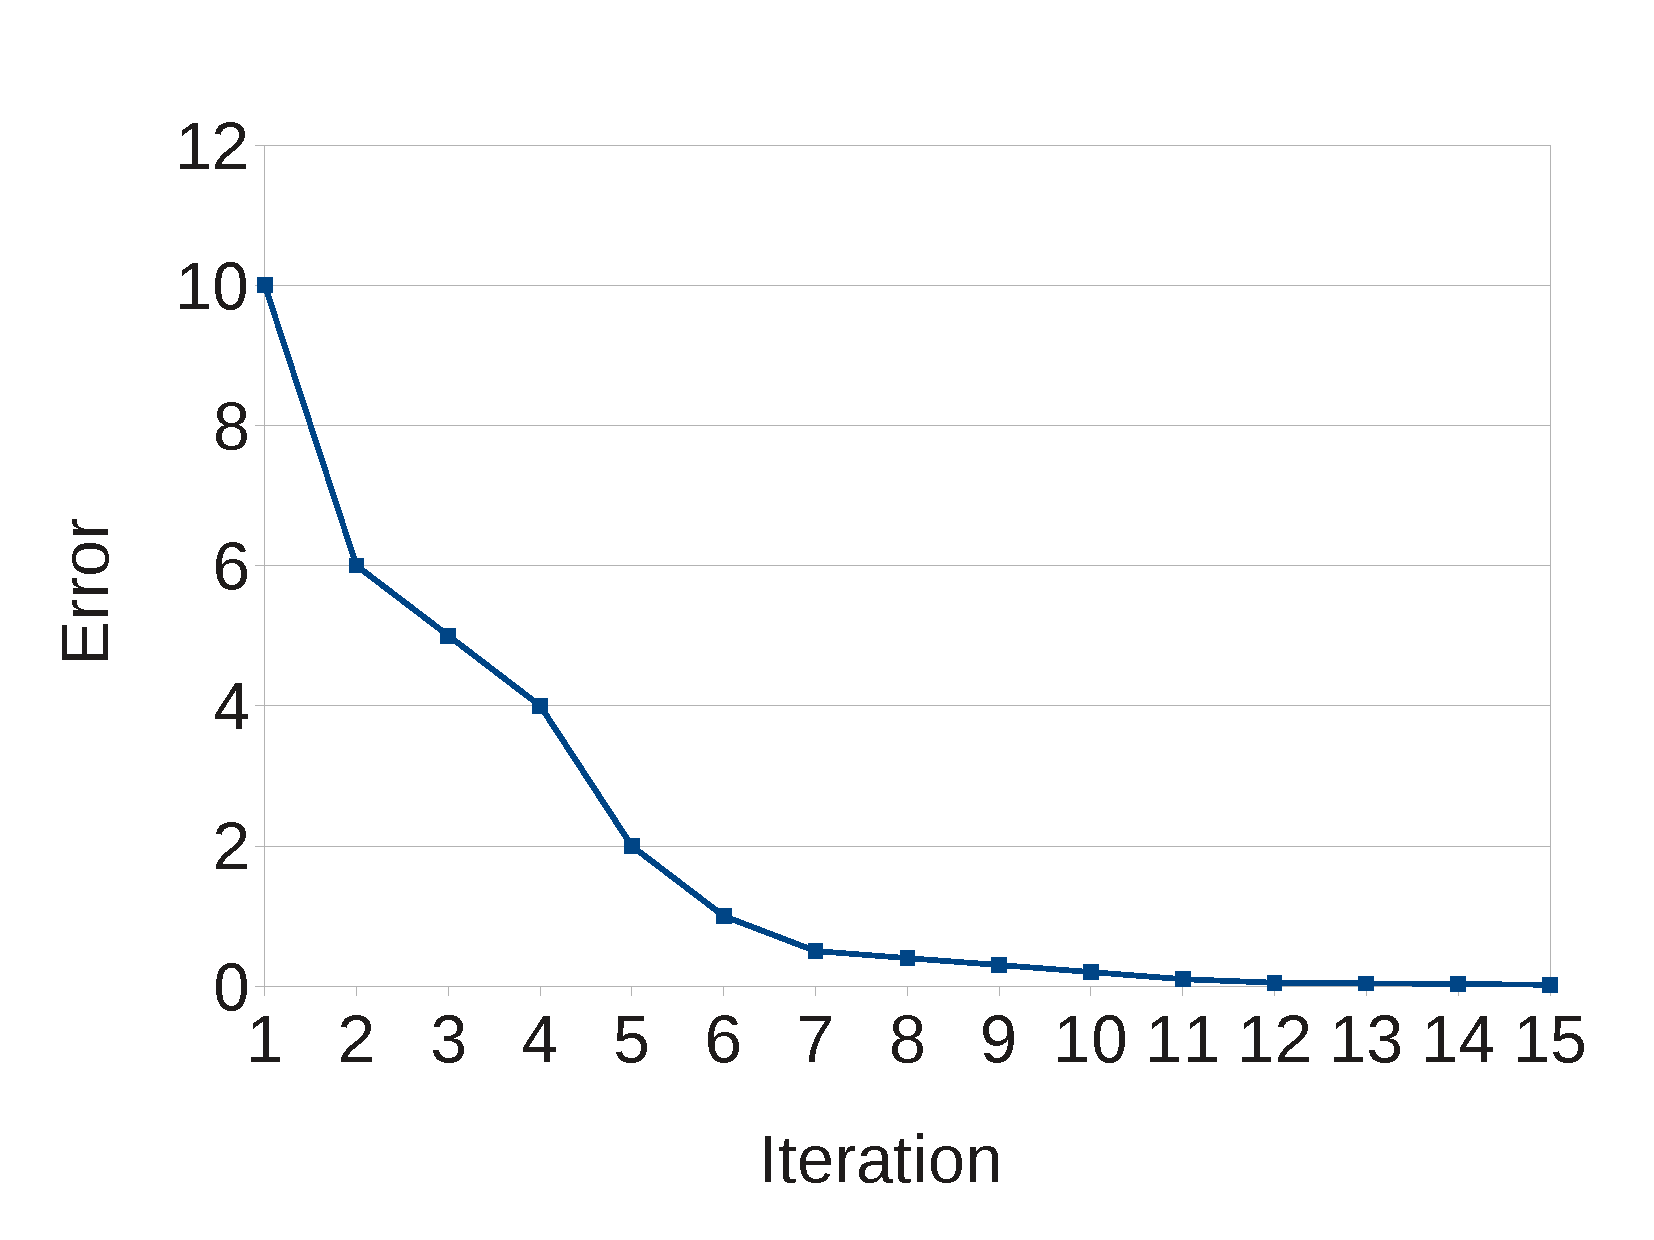
\includegraphics[width=\textwidth]{figure/error.pdf}
    \caption{}
    \label{fig:deformErr}
\end{subfigure}
\caption{Error plots for 
optimizing subsurface-scattering and deformation properties 
iteratively. (a)Subsurface scattering errors. (b)Deformation errors.}
\label{fig:err}
\end{figure}

\subsection{Textured Model}
Input: a textured 3D model and
	measured Albedo of print material.

Output: (Probably gray-scale) Material arranged for different printers in different formats: STL, fable,Gcode.

Printers: Our printer, Makerbot, Objet, maybe Zcorp.

We expand gamut of printable colors by stacking translucent materials. We then applied
dithering with our expanded colors.
\subsection{New Examples for Mechanical Properties}
Ball bounce to certain height. 

A plot of bounce height after each iteration.
The height and desired height is plotted in Figure~\ref{fig:ball}
\begin{figure}
	\centering
 	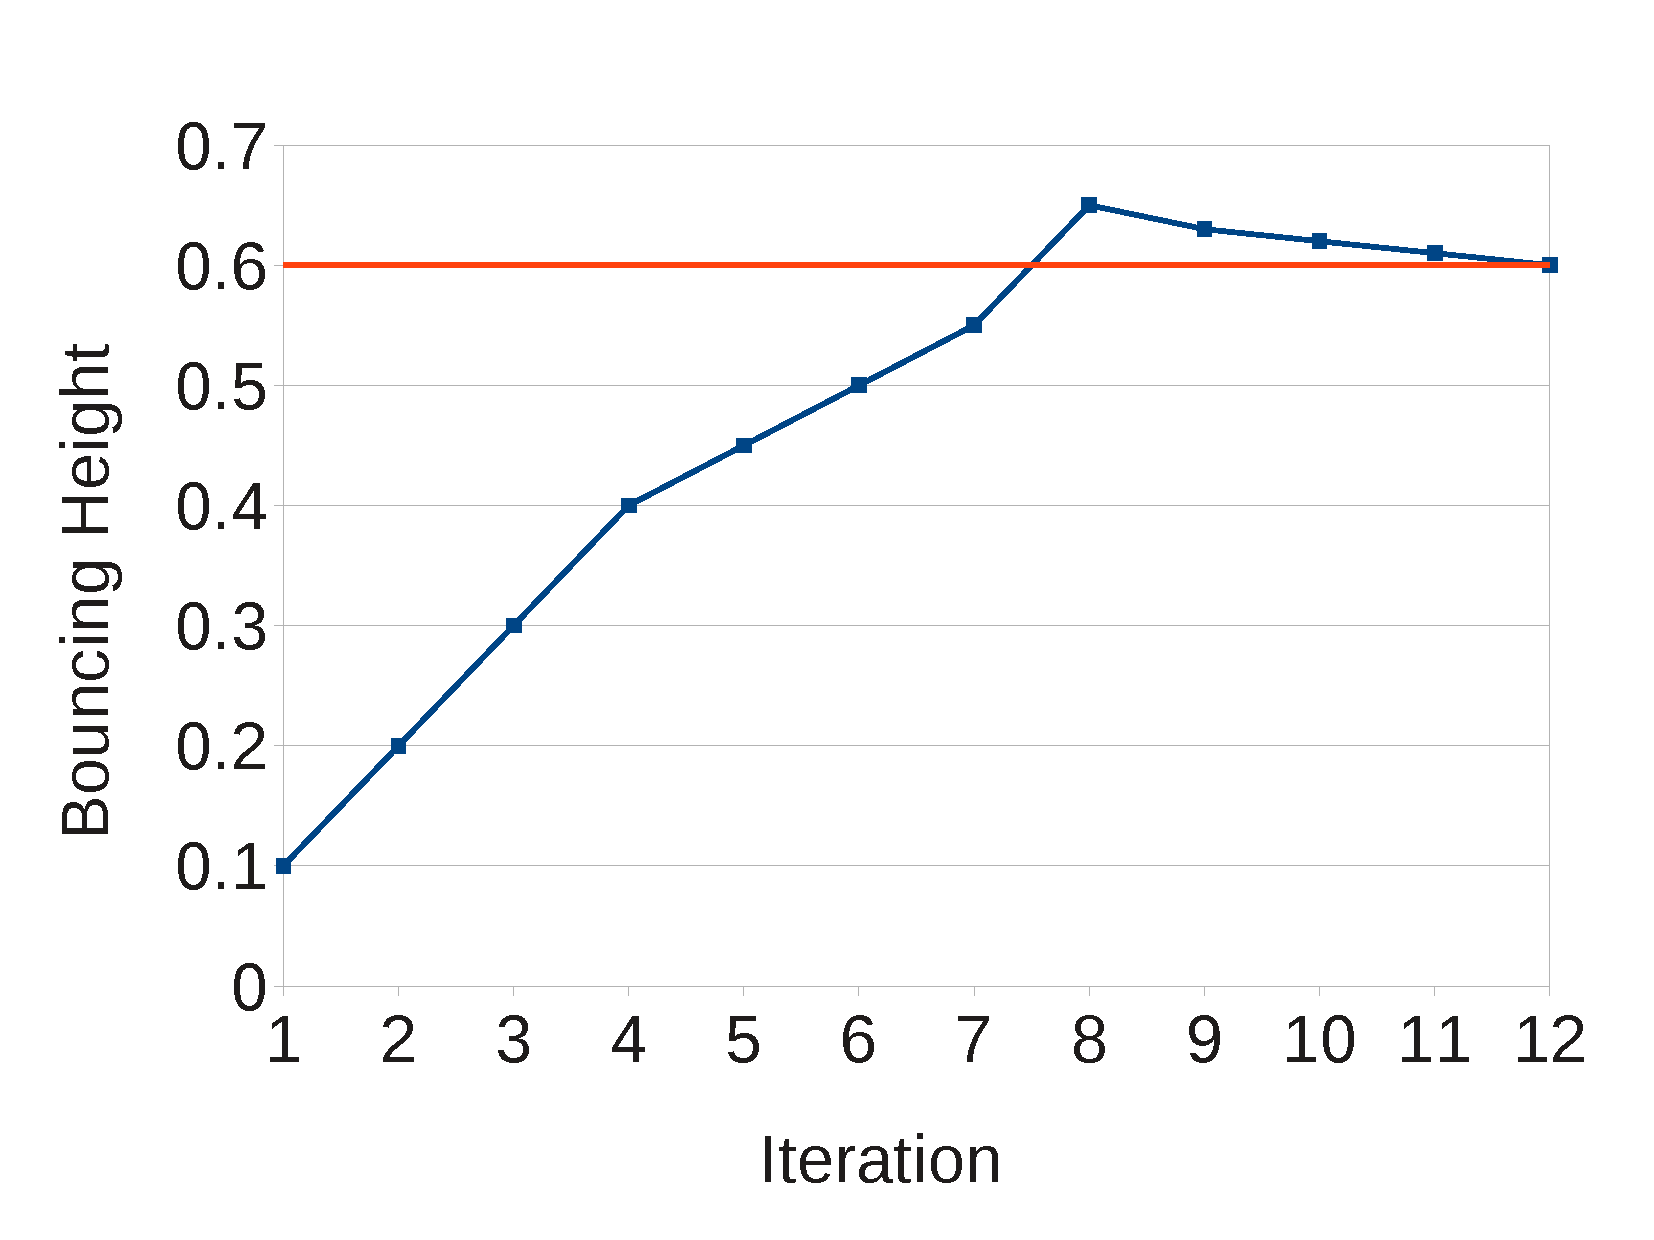
\includegraphics[width=0.3\textwidth]{figure/ballHeight.pdf}
\caption{Simulated height per-iteration of a ball bouncing after free-falling at 1 meter height.
	Redline is desired height.}
\label{fig:ball}
\end{figure}


A loaded die as shown in Figure~\ref{fig:die}. 
\begin{figure}
	\centering
 	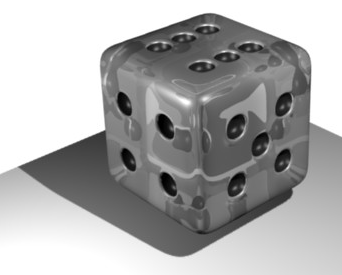
\includegraphics[width=0.25\textwidth]{figure/die.png}
\caption{A printed loaded die}
\label{fig:die}
\end{figure}
It has a certain probability to land on "1".
A table of probability distribution of landing on each side
is shown in Table~\ref{tab:dice}.

\begin{table}
\centering
  \begin{tabular}{ |c| p{0.7in} | p{0.7in} | }
  \hline
  face & simulated probability & measured probability\\
  \hline
  1 & 0.5 & 0.5\\
  \hline
  2 & 0.1 & 0.1\\
  \hline
  3 & 0.1 & 0.1\\
  \hline
  4 & 0.1 & 0.1\\
  \hline
  5 & 0.1 & 0.1\\
  \hline
  6 & 0.1 & 0.1\\

  \hline
  \end{tabular}
  \caption{Simulated and measured dice probability}
  \label{tab:dice}
\end{table}

A plot of simulated probability of landing on "1" after each iteration.

Printer:objet, ours.

\section{Possible Extension}
UI to specify input deformation.
\section{Conclusion}
\section*{Acknowledgements}

\bibliographystyle{acmsiggraph}
\bibliography{paper}
\end{document}
